% !TeX root = ../main.tex

\section{Homework \#2 [2025-09-09]}

\begin{problem}
  Prove
  \[
    \hat H_\text{int} = \frac12 \int \d x \int \d x' v(x,x')
                        \hat n(x) \hat n(x')
                      - \frac12 \int \d x v(x,x) \hat n(x),
  \]
  from $\hat H_\text{int} \ket|x_1 \ldots x_n>
  = \ab(\frac12 \sum_{i\neq j} v(x_i,x_j)) \ket|x_1 \ldots x_N>$
  as hinted in class, beginnning with inserting\linebreak
  $\int \d x \sum_i \delta(x - x_i)$ to the original,
  first-quantization expression and make use of Eq. (3.8.5).
  \begin{equation}
    \begin{aligned}
      \hat n(x) \underbrace{
        \hat\psi^\dagger(x_N) \hat\psi^\dagger(x_{N-1}) \ldots
        \hat\psi^\dagger(x_1) \ket|0>}_{\ket|x_1\ldots x_N>}
  & = [\hat n(x), \hat\psi^\dagger(x_N)]_-
      \hat\psi(x_{N-1}) \ldots \hat\psi^\dagger(x_1) \ket|0>\\
  & + \hat\psi^\dagger(x_N) [\hat n(x), \hat\psi^\dagger(x_{N-1})]_- \ldots
      \hat\psi^\dagger(x_1) \ket|0>\\
  & \vdotswithin =\\
  & + \hat\psi^\dagger(x_N) \hat\psi^\dagger(x_{N-1}) \ldots
      [\hat n(x), \hat\psi^\dagger(x_1)]_- \ket|0>\\
  & = \underbrace{\ab(\sum_{i=1}^N \delta(x - x_i))}_
      {\substack{\text{density of $N$ particles}\\
                 \text{in $x_1$, \ldots\,,~$x_N$}}}
      \ket|x_1 \ldots x_N>.
    \end{aligned}
    \tag{3.8.5}\label{3.8.5}
  \end{equation}
\end{problem}
\begin{solution}
\begin{proof}
  Rewrite the first-quantized interaction
  $\frac12 \sum_{i\neq j} v(x_i,x_j)$ first: separate it into two terms 
  \[
    \sum_{i\neq j} v(x_i,x_j) = \sum_{i,j} v(x_i,x_j) - \sum_{i} v(x_i,x_i),
  \]
  then inserting $\int \d x \sum_i \delta(x - x_i)$ to the two terms above
  \begin{align*}
    \sum_{i,j} v(x_i,x_j) &
  = \int \d x \int \d x' v(x,x')
    \sum_i \delta(x - x_i) \sum_j \delta(x' - x_j),\\
    \sum_{i} v(x_i,x_i)   & = \int \d x v(x,x) \sum_i \delta(x - x_i).
  \end{align*}
  To simplify, define $\ket|\mathcal X> = \ket|x_1 \ldots x_N>
  = \hat\psi^\dagger(x_N) \ldots \hat\psi^\dagger(x_1) \ket|0>$.
  \begin{enumerate}
    \item To generate the first term of $\hat H_\text{int}$,
    acting $\hat n(x)$ and $\hat n(x')$ on $\ket|\mathcal X>$,
    and use the eigenvalue of \eqref{3.8.5}
    \[
      \hat n(x') \hat n(x) \ket|\mathcal X>
    = \sum_i \delta(x - x_i) \sum_j \delta(x' - x_j)
      \ket|\mathcal X>,
    \]
    then multiply $v(x,x')$ and integrate over $x$ and $x'$
    and using the sifting property of $\delta$-function
    \[
      \begin{aligned}
        \int \d x \int \d x' v(x,x') \hat n(x) \hat n(x') \ket|\mathcal X>
    & = \int \d x \int \d x' v(x,x') \sum_i \delta(x - x_i)
        \sum_j \delta(x' - x_j) \ket|\mathcal X>\\
    & = \sum_{i,j} v(x_i,x_j) \ket|\mathcal X>,
      \end{aligned}
    \]
    match the first term of $\hat H_\text{int}$.
    \item Concerning the second term of $\hat H_\text{int}$,
    acting $\hat n(x)$ on $\ket|\mathcal X>$,
    then multiply $v(x,x)$ and integrate over $x$
    \[
      \int \d x v(x,x) \hat n(x) \ket|\mathcal X>
    = \int \d x v(x,x) \sum_i \delta(x - x_i) \ket|\mathcal X> = \sum_i v(x_i,x_i) \ket|\mathcal X>.
    \]
  \end{enumerate}
  In summary,
  \begin{align*}
    \ab(\frac12 \int \d x \d x' v(x,x') \hat n(x) \hat n(x')
  - \frac12 \int \d x v(x,x) \hat n(x)) \ket|\mathcal X>
& = \frac12 \ab(\sum_{i,j} v(x_i,x_j) - \sum_i v(x_i,x_i)) \ket|\mathcal X>\\
& = \frac12 \sum_{i\neq j} v(x_i,x_j) \ket|\mathcal X>.
  \end{align*}
  Then we arrive at
  \[
    \hat H_\text{int} =
    \frac12 \int \d x \d x' v(x,x') \hat n(x) \hat n(x')
  - \frac12 \int \d x v(x,x) \hat n(x).
  \]
\end{proof}
\end{solution}

\begin{problem}[Exercise 1.4 of \cite{4_stefanucci2013nonequilibrium}]
  Let $\hat n_n \equiv \hat d_n^\dagger \hat d_n$
  be the occupation operator for particles with quantum number $n$, see (1.74).
  Prove that in the fermionic case
  \[
    \hat n_n^2 = \hat n_n.
  \]
  and hence that the eigenvalues of $\hat n_n$ are either $0$ or $1$ ---
  that is,
  it is not possible to create two fermions in the same state $\ket|n>$.
  This is a direct consequence of the Pauli exclusion principle.
\end{problem}
\begin{solution}
\begin{proof}
  As is known to all, for fermions,
  the creation and annihilation operators satisfy the following relations
  \[
    \begin{cases}
      \{\hat d_n, \hat d_n^\dagger\}
    = \hat d_n \hat d_n^\dagger + \hat d_n^\dagger \hat d_n = 1,\\
      \{\hat d_n, \hat d_n\} = 0 \Rightarrow \hat d_n \hat d_n = 0,\\
      \{\hat d_n^\dagger, \hat d_n^\dagger\} = 0
      \Rightarrow \hat d_n^\dagger \hat d_n^\dagger = 0.\
    \end{cases}
  \]
  Now calculating $\hat n_n^2$
  \[
    \hat n_n^2 = \hat d_n^\dagger \hat d_n \hat d_n^\dagger \hat d_n
  = \hat d_n^\dagger (1 - \hat d_n^\dagger \hat d_n) \hat d_n
  = \hat d_n^\dagger \hat d_n
  - \hat d_n^\dagger \hat d_n^\dagger \hat d_n \hat d_n
  = \hat d_n^\dagger \hat d_n = \hat n.
  \]
\end{proof}
\begin{proof}
  The eigenfunctions for $\hat n_n$ and $\hat n_n^2$ are
  \[
    \hat n_n \ket|\psi> = \lambda \ket|\psi>, \qq{and}
    \hat n_n^2 \ket|\psi> = \lambda^2 \ket|\psi>.
  \]
  Since $\hat n_n^2 = \hat n_n$, we have
  \[
    \hat n_n\ket|\psi> = \lambda^2 \ket|\psi>.
  \]
  Thus, $\lambda = \lambda^2$ and $\lambda = 0$ or $1$,
  means it is impossible to have more than one fermion
  in the same quantum state $\ket|n>$, which is the Pauli exclusion principle.
\end{proof}
\end{solution}

\begin{problem}[Exercise 1.5 of \cite{4_stefanucci2013nonequilibrium}]
  Prove that the total number of particle operators
  $\hat N = \int \d x \hat\psi^\dagger(x) \hat\psi(x)$
  can also be written as $\hat N = \sum_n \hat d_n^\dagger \hat d_n$
  for any orthonormal basis $\ket|n>$.
  Calculate the action of $\hat N$ on a generic ket $\ket|\Psi_N>$
  with $N$ particles ($\ket|\Psi_N> \in H_N$) and prove that
  \[
    \hat N \ket|\Psi_N> = N \ket|\Psi_N>.
  \]
\end{problem}
\begin{solution}
\begin{proof}
  Recalling the definitions of the field operators
  \begin{align*}
    \hat\psi(x) & = \sum_n \braket<x|n> \hat d_n = \sum_n \phi_n(x) \hat d_n,\\
    \hat\psi(x)^\dagger & = \sum_n \braket<n|x> \hat d_n^\dagger
  = \sum_n \phi_n^*(x) \hat d_n^\dagger.
  \end{align*}
  then substitute them into $\hat N$ and use the orthonormality of $\{\ket|n>\}$
  \begin{align*}
    \hat N & = \int \d x \hat\psi^\dagger(x) \hat\psi(x)
  = \int \d x \sum_m \phi_m^*(x) \hat d_m^\dagger
              \sum_n \phi_n(x) \hat d_n^\dagger\\
& = \sum_{m,n} \hat d_m^\dagger \hat d_n \int \d x \phi_m^*(x) \phi_n(x)
  = \sum_{m,n} \hat d_m^\dagger \hat d_n \delta_{m,n}
  = \sum_n \hat d_n^\dagger \hat d_n,
  \end{align*}
  means that $\hat N$ can be written as
  $\hat N = \sum_n \hat d_n^\dagger \hat d_n$
  for any orthonormal basis $\ket|n>$.
\end{proof}
\begin{proof}
  When $\hat N$ act on $\ket|\Psi_N>$
  \[
    \hat N \ket|\Psi_N>
  = \int \d x \hat\psi(x)^\dagger \hat\psi(x) \ket|x_1, x_2, \ldots,x_N>
  = \int \d x \sum_{i=1}^N \delta(x - x_i) \ket|x_1, x_2, \ldots,x_N>
  = N \ket|x_1, x_2, \ldots,x_N>,
  \]
  So, we proved that $\hat N \ket|\Psi_N> = N \ket|\Psi_N>$.
\end{proof}
\end{solution}

\begin{framed}
  \justifying \noindent
  The total Hamiltonian of a system of interacting identical particles
  is the sum of $\hat H_0$ and $\hat H_\text{int}$.
  Expressing $\hat H$ in terms of the $\hat d$-operators as
  $\hat H = \hat H_0 + \hat H_\text{int}
  = \sum_{ij} h_{ij} \hat d_i^\dagger \hat d_j
  + \frac12 \sum_{ij,n} v_{ijmn} \hat d_i^\dagger \hat d_j^\dagger
    \hat d_m \hat d_n$.
\end{framed}
\begin{problem}[Exercise 1.6 of \cite{4_stefanucci2013nonequilibrium}]
  Prove that $\hat N$ commutes with $\hat H_0$ and $\hat H_\text{int}$ ---
  that is,
  \[
    [\hat N, \hat H_0]_- = [\hat N, \hat H_\text{int}]_- = 0.
  \]
  This means that the eigenkets of $\hat H$
  can be chosen as kets with a fixed number of particles.
\end{problem}
\begin{solution}
\begin{proof}
  Since the annihilation operator $\hat d_m$ destorys a particle,
  so it decreases the number by $1$: $[\hat N, \hat d_m] = -\hat d_m$;
  in contrast, the creation operator $\hat d_m^\dagger$ creates a particle,
  so $[\hat N, \hat d_m^\dagger] = \hat d_m^\dagger$. Then
  \begin{align*}
    [\hat N, \hat H_0] & = \hat N \hat H_0 - \hat H_0 \hat N
  = \sum_{ij} h_{ij} [\hat N, \hat d_i^\dagger \hat d_j]
  = \sum_{ij} h_{ij} \hat d_i^\dagger [\hat N, \hat d_j]
  + \sum_{ij} h_{ij} [\hat N, \hat d_i^\dagger]\hat d_j\\
  & = \hat d_i^\dagger (-\hat d_j) + (\hat d_i^\dagger) \hat d_j = 0,
  \end{align*}
  similarly, since
  \[
    [\hat N, \hat d_i^\dagger \hat d_j^\dagger \hat d_m \hat d_n]
  = (\hat d_i^\dagger) \hat d_j^\dagger \hat d_m \hat d_n
  + \hat d_i^\dagger (\hat d_j^\dagger) \hat d_m \hat d_n
  + \hat d_i^\dagger \hat d_j^\dagger (-\hat d_m) \hat d_n
  + \hat d_i^\dagger \hat d_j^\dagger \hat d_m (-\hat d_n) = 0,
  \]
  we arrive at $[\hat N, \hat H_\text{int}] = 0$.
\end{proof}
\end{solution}

\begin{problem}[Exercise 1.7 of \cite{4_stefanucci2013nonequilibrium}]
  Let $n = s\sigma$ and $\sigma = \uparrow,\downarrow$
  be the spin projection for fermions of spin $\frac12$.
  We consider the operators
  \[
    \hat S_s^z \equiv \frac12 (\hat n_{s\uparrow} - \hat n_{s\downarrow}),~
    \hat S_s^+ \equiv \hat d_{s\uparrow}^\dagger \hat d_{s\downarrow},~
    \hat S_s^- \equiv \hat d_{s\downarrow}^\dagger \hat d_{s\uparrow}
  = (\hat S_s^+)^\dagger.
  \]
  Using the anticommutation relations,
  \begin{framed}
  \[
    \{\hat d_{s\sigma}, \hat d_{s'\sigma'}^\dagger\}
  = \delta_{ss'} \delta_{\sigma\sigma'},~
    \{\hat d_{s\sigma}, \hat d_{s'\sigma'}\} = 0,~
    \{\hat d_{s\sigma}^\dagger, \hat d_{s'\sigma'}^\dagger\} = 0.
  \]
  \end{framed}
  prove that the action of
  the above operators on the kets
  $\ket|s\sigma> \equiv \hat d_{s\sigma}^\dagger \ket|0>$ is
  \[
    \hat S_s^z \ket|s\uparrow> = \frac12 \ket|s\uparrow>,~
    \hat S_s^+ \ket|s\uparrow> = \ket|\emptyset>,~
    \hat S_s^- \ket|s\uparrow> = \ket|s\downarrow>,
  \]
  and
  \[
    \hat S_s^z \ket|s\downarrow> = -\frac12 \ket|s\downarrow>,~
    \hat S_s^+ \ket|s\downarrow> = \ket|s\uparrow>,~
    \hat S_s^- \ket|s\downarrow> = \ket|\emptyset>,
  \]
  To what operator do $\hat S_s^z$, $\hat S_s^+$, $\hat S_s^-$ correspond?
\end{problem}
\begin{solution}
  Using the occupation operator
  $\hat n_{s\sigma} = \hat d_{s\sigma}^\dagger \hat d_{s\sigma}$
  and the relation $\hat d_{s\sigma}\ket|0> = 0$,
  $\hat d_{s\sigma}^\dagger = \ket|s\sigma>$.
  \begin{enumerate}
    \item $\hat S_s^z \ket|s\uparrow>
  = \frac12(\hat d_{s\uparrow}^\dagger \hat d_{s\uparrow}
            \hat d_{s\uparrow}^\dagger -
            \hat d_{s\downarrow}^\dagger \hat d_{s\downarrow}
            \hat d_{s\uparrow}^\dagger)\ket|0>
  = \frac12[\hat d_{s\uparrow}^\dagger
            (1 -  \hat d_{s\uparrow}^\dagger
                  \hat d_{s\uparrow}) -
            (-\hat d_{s\downarrow}^\dagger
            \hat d_{s\uparrow}^\dagger \hat d_{s\downarrow})]\ket|0>
  = \frac12 \ket|s\uparrow>$. \hfill\qedsymbol
    \item $\hat S_s^+ \ket|0>
  = \hat d_{s\uparrow}^\dagger \hat d_{s\downarrow}
    \hat d_{s\uparrow}^\dagger \ket |0>
  = -\hat d_{s\uparrow}^\dagger \hat d_{s\uparrow}^\dagger
    \hat d_{s\downarrow} \ket |0> = 0$,
    so $\hat S_s^+ \ket|s\uparrow> = \ket|\emptyset>$.\hfill\qedsymbol
    \item $\hat S_s^- \ket|s\uparrow>
  = \hat d_{s\downarrow}^\dagger \hat d_{s\uparrow}
    \hat d_{s\uparrow}^\dagger \ket|0>
  = \hat d_{s\downarrow}^\dagger
    (1 - \hat d_{s\uparrow}^\dagger \hat d_{s\uparrow}) \ket|0>
  = \ket|s\downarrow>$.\hfill\qedsymbol
    \item $\hat S_s^z \ket|s\downarrow>
  = \frac12(\hat d_{s\uparrow}^\dagger \hat d_{s\uparrow}
            \hat d_{s\downarrow}^\dagger -
            \hat d_{s\downarrow}^\dagger \hat d_{s\downarrow}
            \hat d_{s\downarrow}^\dagger)\ket|0>
  = \frac12[-\hat d_{s\uparrow}^\dagger \hat d_{s\downarrow}^\dagger
            \hat d_{s\uparrow} - \hat d_{s\downarrow}^\dagger
            (1 - \hat d_{s\downarrow}^\dagger \hat d_{s\downarrow})]\ket|0>
  = -\frac12 \ket|s\downarrow>$.\hfill\qedsymbol
    \item $\hat S_s^+ \ket|s\downarrow>
  = \hat d_{s\uparrow}^\dagger \hat d_{s\downarrow}
    \hat d_{s\downarrow}^\dagger \ket |0>
  = \hat d_{s\uparrow}^\dagger
    (1 - \hat d_{s\downarrow}^\dagger \hat d_{s\downarrow}) \ket |0>
  = \ket|s\uparrow>$.\hfill\qedsymbol
    \item $\hat S_s^- \ket|0>
  = \hat d_{s\downarrow}^\dagger \hat d_{s\uparrow}
    \hat d_{s\downarrow}^\dagger \ket |0>
  = - \hat d_{s\downarrow}^\dagger \hat d_{s\downarrow}^\dagger 
    \hat d_{s\uparrow} \ket |0> = 0$,
    so $\hat S_s^- \ket|s\downarrow> = \ket|\emptyset>$.\hfill\qedsymbol
  \end{enumerate}
  The operators $\hat S_s^z$, $\hat S_s^+$, and $\hat S_s^-$
  correspond to the spin operators
  \begin{itemize}
    \item Since $\hat S_s^z$ will not change the state, just ``returns''
    different eigenvalues, so it measures the $z$-component of spin.
    \item Since $\hat S_s^+$ annihilates $\ket|\uparrow>$
    and raises $\ket|\downarrow>$ to $\ket|\uparrow>$,
    so it is the raising operator.
    \item Since $\hat S_s^-$ lowers $\ket|\uparrow>$
    and annihilates $\ket|\downarrow>$,
    so it is the lowering operator.
  \end{itemize}
\end{solution}

\begin{problem}[Exercise 1.8 of \cite{4_stefanucci2013nonequilibrium}]
  Let us define the spin operators along the $x$ and $y$ directions as
  \[
    \hat S_s^x \equiv \frac12(\hat S_s^+ + \hat S_s^-),~
    \hat S_y^x \equiv \frac1{2\iu}(\hat S_s^+ - \hat S_s^-),
  \]
  and the spin operator $\hat S_s^z$ along the $z$ direction as in (1.91).
  Prove that these operators can also be written as
  \[
    \hat S_s^j = \frac12 \sum_{\sigma\sigma'}
    \hat d_{s\sigma}^\dagger \sigma_{\sigma\sigma'}^j \hat d_{s\sigma'},~
    j = x, y, z
  \]
  with
  \[
    \sigma^x =
    \begin{pmatrix}
      0 & 1\\
      1 & 0
    \end{pmatrix},~
    \sigma^y =
    \begin{pmatrix}
      0 & -\iu\\
      \iu & 0
    \end{pmatrix},~
    \sigma^z =
    \begin{pmatrix}
      1 & 0\\
      0 & -1
    \end{pmatrix},
  \]
  the Pauli matrices. Using the anticommutation relations, verify that
  \[
    [\hat S_s^i, \hat S_{s'}^j]_- =
    \iu \delta_{ss'} \sum_{k=x,y,z} \epsilon_{ijk} \hat S_s^k,
  \]
  where $\epsilon_{ijk}$ is the Levi-Civita tensor.
\end{problem}
\begin{solution}
\begin{proof}
  Verify every directions: $x$, $y$, $z$ respectively.
    \begin{align*}
  \intertext{For $j = x$}
    \frac12 \sum_{\sigma,\sigma'} \hat d_{s\sigma}^\dagger
    \sigma_{\sigma\sigma'}^x \hat d_{s\sigma'}
  & = \frac12 \ab[\hat d_{s\uparrow}^\dagger(0) \hat d_{s\uparrow}
                + \hat d_{s\uparrow}^\dagger(1) \hat d_{s\downarrow}
                + \hat d_{s\downarrow}^\dagger(1) \hat d_{s\uparrow}
                + \hat d_{s\downarrow}^\dagger(0) \hat d_{s\downarrow}]\\
  & = \frac12 (\hat d_{s\uparrow}^\dagger \hat d_{s\downarrow}
    + \hat d_{s\downarrow}^\dagger \hat d_{s\uparrow}) = \hat S_s^x,\\
  \intertext{similarly, for $j = y$ and $j = z$}
    \frac12 \sum_{\sigma,\sigma'} \hat d_{s\sigma}^\dagger
    \sigma_{\sigma\sigma'}^y \hat d_{s\sigma'}
  & = \frac12 \ab[ \hat d_{s\uparrow}^\dagger(0) \hat d_{s\uparrow}
    + \hat d_{s\uparrow}^\dagger (-\iu) \hat d_{s\downarrow}
    + \hat d_{s\downarrow}^\dagger (\iu) \hat d_{s\uparrow}
    + \hat d_{s\downarrow}^\dagger(0) \hat d_{s\downarrow}]
    = \hat S_s^y,\\
    \frac12 \sum_{\sigma,\sigma'} \hat d_{s\sigma}^\dagger
    \sigma_{\sigma\sigma'}^z \hat d_{s\sigma'}
  & = \frac12 \ab[\hat d_{s\uparrow}^\dagger(1) \hat d_{s\uparrow}
                + \hat d_{s\uparrow}^\dagger(0) \hat d_{s\downarrow}
                + \hat d_{s\downarrow}^\dagger(0) \hat d_{s\uparrow}
                + \hat d_{s\downarrow}^\dagger (-1) \hat d_{s\downarrow}]
    = \hat S_s^z.
    \end{align*}
  Then, $\hat S_s^j = \frac12 \sum_{\sigma\sigma'}
    \hat d_{s\sigma}^\dagger \sigma_{\sigma\sigma'}^j \hat d_{s\sigma'},~
    j = x, y, z$ is valid.
\end{proof}
  Consider the simple situation $s' = s$, that is
  \[
    [\hat S_s^i, \hat S_s^j] = \iu \sum_{k} \epsilon_{ijk} \hat S_s^k.
  \]
  Write $\hat S_s^i$, $\hat S_s^j$ in terms of the representation just proved
  \[
    \hat S_s^i = \frac12 \sum_{\alpha\beta}
    \hat d_{s\alpha}^\dagger \sigma_{\alpha\beta}^i \hat d_{s\beta}, \quad
    \hat S_s^j = \frac12 \sum_{\gamma\delta}
    \hat d_{s\gamma}^\dagger \sigma_{\gamma\delta}^j \hat d_{s\delta}.
  \]
  and substitute them into the commutator
  \[
    [\hat S_s^i, \hat S_s^j]
  = \hat S_s^i \hat S_s^j - \hat S_s^j \hat S_s^i
  = \frac14 \sum_{\alpha\beta\gamma\delta}
    \ab[
      \hat d_{s\alpha}^\dagger \sigma_{\alpha\beta}^i \hat d_{s\beta}
      \hat d_{s\gamma}^\dagger \sigma_{\gamma\delta}^j \hat d_{s\delta}
    - \hat d_{s\gamma}^\dagger \sigma_{\gamma\delta}^j \hat d_{s\delta}
      \hat d_{s\alpha}^\dagger \sigma_{\alpha\beta}^i \hat d_{s\beta}].
  \]
  Consider the product
  $\hat d_{s\beta} \hat d_{s\gamma}^\dagger =
  \delta_{\beta\gamma} - \hat d_{s\gamma}^\dagger \hat d_{s\beta}$
  and the relation
  $\delta_{\beta\gamma} \sigma_{\gamma\delta}^j = \sigma_{\beta\delta}^j$,
  the first term gets
  \begin{align*}
    \hat d_{s\alpha}^\dagger \sigma_{\alpha\beta}^i \hat d_{s\beta}
    \hat d_{s\gamma}^\dagger \sigma_{\gamma\delta}^j \hat d_{s\delta}
& = \hat d_{s\alpha}^\dagger \sigma_{\alpha\beta}^i
    [\delta_{\beta\gamma} - \hat d_{s\gamma}^\dagger \hat d_{s\beta}]
    \sigma_{\gamma\delta}^j \hat d_{s\delta}
  = \hat d_{s\alpha}^\dagger \sigma_{\alpha\beta}^i \delta_{\beta\gamma}
    \sigma_{\gamma\delta}^j \hat d_{s\delta}
  - \hat d_{s\alpha}^\dagger \sigma_{\alpha\beta}^i \hat d_{s\gamma}^\dagger
    \hat d_{s\beta} \sigma_{\gamma\delta}^j \hat d_{s\delta}\\
& = \hat d_{s\alpha}^\dagger \sigma_{\alpha\beta}^i
    \sigma_{\beta\delta}^j \hat d_{s\delta}
  - \hat d_{s\alpha}^\dagger \sigma_{\alpha\beta}^i \hat d_{s\gamma}^\dagger
    \hat d_{s\beta} \sigma_{\gamma\delta}^j \hat d_{s\delta},\\
  \intertext{similarly, for the other term in the commutator}
    \hat d_{s\gamma}^\dagger \sigma_{\gamma\delta}^j \hat d_{s\delta}
    \hat d_{s\alpha}^\dagger \sigma_{\alpha\beta}^i \hat d_{s\beta}
& = \hat d_{s\gamma}^\dagger \sigma_{\gamma\delta}^j
    [\delta_{\delta\alpha} - \hat d_{s\alpha}^\dagger \hat d_{s\delta}]
    \sigma_{\alpha\beta}^i \hat d_{s\beta}
  = \hat d_{s\gamma}^\dagger \sigma_{\gamma\delta}^j
    \sigma_{\delta\beta}^i \hat d_{s\beta}
  - \hat d_{s\gamma}^\dagger \sigma_{\gamma\delta}^j \hat d_{s\alpha}^\dagger
    \hat d_{s\delta} \sigma_{\alpha\beta}^i \hat d_{s\beta}.
  \end{align*}
  The terms with four operators cancel,
  since the spin operators are bilinear in fermions
  and the commutation should be close to bilinear.
  
  For the situation $s \neq s'$,
  the operators commute because they act on different sites.
  So a $\delta$-function will be inserted. Therefore
  \begin{align*}
    [\hat S_s^i, \hat S_s^j]
  & = \frac14 \sum_{\alpha\beta} \hat d_{s\alpha}^\dagger
      [\sigma^i, \sigma^j]_{\alpha\beta} \hat d_{s\beta}
    = \frac14 \sum_{\alpha\beta} \hat d_{s\alpha}^\dagger
      \ab\bigg(2i \sum_k \epsilon_{ijk} \sigma^k)_{\alpha\beta}
      \hat d_{s\beta}\\
  & = \frac\iu2 \sum_k \epsilon_{ijk} \sum_{\alpha\beta}
      \hat d_{s\alpha}^\dagger \sigma_{\alpha\beta}^k \hat d_{s\beta}
    = i \sum_k \epsilon_{ijk} \hat S_s^k.
  \end{align*}
\end{solution}

\begin{problem}[Exercise 2.2 of \cite{4_stefanucci2013nonequilibrium}]
  Consider the one-dimensional crystal below,
  \begin{center}
    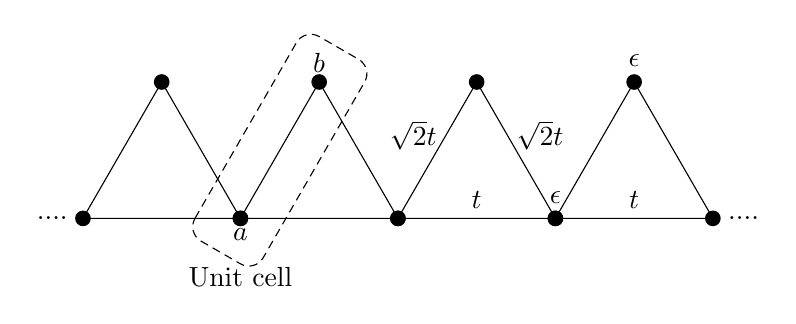
\begin{tikzpicture}
      \draw (0,0) node [circle, fill, inner sep = 2pt] {}
       node [left = 2pt] {....} --
            (2,0) node [circle, fill, inner sep = 2pt] {} --
            (1,{sqrt(3)}) node [circle, fill, inner sep = 2pt] {} -- cycle;
      \draw (2,0) node [circle, fill, inner sep = 2pt] {} --
            (4,0) node [circle, fill, inner sep = 2pt] {} --
            (3,{sqrt(3)}) node [circle, fill, inner sep = 2pt] {}
       coordinate [label = above:$b$] (b) -- cycle
       coordinate [label = below:$a$] (a);
      \draw (4,0) node [circle, fill, inner sep = 2pt] {} --
            (6,0) node [circle, fill, inner sep = 2pt] {}
       node [above = 2pt] {$\epsilon$} node [midway, above] {$t$} --
            (5,{sqrt(3)}) node [circle, fill, inner sep = 2pt] {}
       node [above right, midway, inner sep = 0pt] {$\sqrt2t$} -- cycle
       node [above left, midway, inner sep = 0pt] {$\sqrt2t$};
      \draw (6,0) node [circle, fill, inner sep = 2pt] {} --
            (8,0) node [circle, fill, inner sep = 2pt] {}
       node [midway, above] {$t$} node [right = 2pt] {....} --
            (7,{sqrt(3)}) node [circle, fill, inner sep = 2pt] {}
       node [above = 2pt] {$\epsilon$} -- cycle;
      \draw [rotate around = {-30:(a)}, rounded corners = 6pt, densely dashed]
        ([xshift = -.5cm, yshift = -.5cm]a) rectangle + (1,3)
       node [below = .5cm] at (a) {Unit cell};
    \end{tikzpicture}
  \end{center}
  with marices $h =
  \begin{psmallmatrix}
    \epsilon & \sqrt2t\\
    \sqrt2t & \epsilon
  \end{psmallmatrix}$ and $T =
  \begin{psmallmatrix}
    t & \sqrt2t\\
    0 & 0
  \end{psmallmatrix}$.
  Show that for $t > 0$ the two bands are
  \begin{align*}
    \epsilon_{k1} & = \epsilon - 2t,\\
    \epsilon_{k2} & = \epsilon + 2t + 2t\cos k,
  \end{align*}
  with $k \in (-\pi,\pi)$.
  The first band is therefore perfectly flat.
  If we have half an electron per unit cell,
  then the ground state is highly degenerate.
  For instance, the states obtained by occupying each $k$-level
  of the flat band with an electron of
  either spin up or down all have the same energy.
  This degeneracy is lifted by the electron-electron interaction
  and the ground state truns out
  to be the one in which all electrons have parallel spins.
  The crystal is then a ferromagnet.
  The ferromagnetism in flat-band crystals was proposed
  by Mielke and Tasaki [11,12,13]
  and is usually called flat-band ferromagnetism.
\end{problem}
\begin{solution}
  For a periodic system, the Bloch Hamiltonian $H(k)$ is
  \[
    \mathcal H(k) = h + T \upe^{\iu k} + T^\dagger \upe^{-\iu k}
  = \begin{pmatrix}
      \epsilon + 2t \cos k & \sqrt2t (1 + \upe^{\iu k}) \\
      \sqrt2t (1 + \upe^{-ik}) & \epsilon
  \end{pmatrix}.
  \]
  To find the eigenvalues $\epsilon_k$,
  let $\det(\mathcal H(k) - \epsilon_k\mathbbm 1) = 0$
  \[
  \begin{vmatrix}
  \epsilon + 2t \cos k - \epsilon_k & \sqrt2t (1 + \upe^{\iu k}) \\
  \sqrt2t (1 + e^{-ik}) & \epsilon - \epsilon_k
  \end{vmatrix} = 0,
  \]
  and let $\Delta = \epsilon_k - \epsilon$ for simplicity. Then we get
  $\Delta_1 = 2t \cos k + 2t$, $\Delta_2 = t \cos k - t (\cos k + 2) = -2t$.
  Thus, the two bands are
  \[
    \epsilon_{k1} = \epsilon - 2t, \quad
    \epsilon_{k2} = \epsilon + 2t + 2t \cos k.
  \]
\end{solution}